\documentclass{article}

% Recommended, but optional, packages for figures and better typesetting:
\usepackage{microtype}
\usepackage{graphicx}
\usepackage{subcaption}
\usepackage{booktabs} % for professional tables

% hyperref makes hyperlinks in the resulting PDF.
% If your build breaks (sometimes temporarily if a hyperlink spans a page)
% please comment out the following usepackage line and replace
% \usepackage{icml2026} with \usepackage[nohyperref]{icml2026} above.
\usepackage{xurl}
\usepackage{hyperref}


% Attempt to make hyperref and algorithmic work together better:
\newcommand{\theHalgorithm}{\arabic{algorithm}}

% Use the following line for the initial blind version submitted for review:
\usepackage[accepted]{icml2026}

% For preprint, use
% \usepackage[preprint]{icml2026}

% If accepted, instead use the following line for the camera-ready submission:
% \usepackage[accepted]{icml2026}

\usepackage{amsmath}
\usepackage{amssymb}
\usepackage{mathtools}
\usepackage{amsthm}
\usepackage{svg}
\usepackage{placeins}
\usepackage{algorithm}
\usepackage{algorithmic}
\usepackage{float}


% if you use cleveref..
\usepackage[capitalize,noabbrev]{cleveref}

%%%%%%%%%%%%%%%%%%%%%%%%%%%%%%%%
% THEOREMS
%%%%%%%%%%%%%%%%%%%%%%%%%%%%%%%%
\theoremstyle{plain}
\newtheorem{theorem}{Theorem}[section]
\newtheorem{proposition}[theorem]{Proposition}
\newtheorem{lemma}[theorem]{Lemma}
\newtheorem{corollary}[theorem]{Corollary}
\theoremstyle{definition}
\newtheorem{definition}[theorem]{Definition}
\newtheorem{assumption}[theorem]{Assumption}
\theoremstyle{remark}
\newtheorem{remark}[theorem]{Remark}

% Todonotes is useful during development; simply uncomment the next line
%    and comment out the line below the next line to turn off comments
%\usepackage[disable,textsize=tiny]{todonotes}
\usepackage[textsize=tiny]{todonotes}


\usepackage{xspace}
\newcommand{\ourmodel}{SMFM\xspace}

% The \icmltitle you define below is probably too long as a header.
% Therefore, a short form for the running title is supplied here:
\icmltitlerunning{\ourmodel: Spectral-Cost Multi-Marginal Flow Matching}

\begin{document}


\twocolumn[
  \icmltitle{\ourmodel: Spectral-Cost Multi-Marginal Flow Matching}

  % It is OKAY to include author information, even for blind submissions: the
  % style file will automatically remove it for you unless you've provided
  % the [accepted] option to the icml2026 package.

  % List of affiliations: The first argument should be a (short) identifier you
  % will use later to specify author affiliations Academic affiliations
  % should list Department, University, City, Region, Country Industry
  % affiliations should list Company, City, Region, Country

  % You can specify symbols, otherwise they are numbered in order. Ideally, you
  % should not use this facility. Affiliations will be numbered in order of
  % appearance and this is the preferred way.
  \icmlsetsymbol{equal}{*}

  \begin{icmlauthorlist}
    \icmlauthor{David Crair}{yale}
  \end{icmlauthorlist}

  \icmlaffiliation{yale}{Yale University}

  \icmlcorrespondingauthor{David Crair}{david.crair@yale.edu}

  % You may provide any keywords that you find helpful for describing your
  % paper; these are used to populate the "keywords" metadata in the PDF but
  % will not be shown in the document
  \icmlkeywords{Machine Learning, ICML}

    \vskip 0.08in
    \begin{center}
    \small
    \textbf{Code:} \href{https://github.com/davidcrair/smfm}
    {\texttt{github.com/davidcrair/smfm}}
    \end{center}

  \vskip 0.3in
]

% this must go after the closing bracket ] following \twocolumn[ ...

% This command actually creates the footnote in the first column listing the
% affiliations and the copyright notice. The command takes one argument, which
% is text to display at the start of the footnote. The \icmlEqualContribution
% command is standard text for equal contribution. Remove it (just {}) if you
% do not need this facility.

% Use ONE of the following lines. DO NOT remove the command.
% If you have no special notice, KEEP empty braces:
\printAffiliationsAndNotice{}  % no special notice (required even if empty)
% Or, if applicable, use the standard equal contribution text:
% \printAffiliationsAndNotice{\icmlEqualContribution}

\begin{abstract}
Flow Matching (FM) is a powerful framework for generative modeling of data. One instance that is particularly relevant for scientific applications is the multi-marginal setting, where there are intermediate data marginals between source and target distributions, with applications in cell differentiation and weather modeling. We introduce a new family of Optimal Transport (OT) costs to the multi-marginal FM problem, adapting pre-existing work in graph-Laplacian spectral distances to pair samples between adjacent marginals during training. This extension preserves simulation-free training while enabling manifold-aware FM couplings. We show a consistent improvement in performance across multiple datasets, compared to a baseline using the standard squared Euclidean distance for OT couplings, when using Spectral distances in OT couplings for Multi-Marginal Flow Matching (\ourmodel).
\end{abstract}

\section{Introduction}
Studying how the trajectories of samples evolve over time in a setting where we have access to snapshots of marginals over time is important in many fields, including in single-cell biology or climate science. The central difficulty is that observations are cross-sectional: samples are often unpaired across marginals, intermediate trajectories are unobserved, and high dimensional measurements often lie along a curved low-dimensional manifold, where standard Euclidean distances can be unreliable. This gives rise to two key considerations and active areas of research: handling the discrete marginal structure of the data and explicitly using the Riemannian manifold-structure of the dataset as a whole.

The main frameworks that have appeared for solving this trajectory inference problem structure are Optimal Transport (OT) and Flow Matching (FM) \cite{lipmanFlowMatchingGenerative2023, liuRectifiedFlowFlow2022}. Flow matching is one common training framework used to learn a vector field that defines an ordinary differential equation (ODE) which can be integrated using an ODE solver to predict flows from source to target distributions. In the trajectory inference problem, it is not just matching the source distribution that is valuable, but also predicting interpolations between marginal distributions that are logical and usable for downstream applications, like causality inference \cite{sunCFlowsRevealingDynamic}. Optimal Transport is used to pair samples in adjacent marginals to stabilize training and increase inference speed but commonly relies on pairing samples to minimize total Euclidean distance (2-Wasserstein) which ignores the manifold-structure of high-dimensional data \cite{tongImprovingGeneralizingFlowbased2024}.

Separately, methods have been develop to interrogate the connectivity and geometric structure of graphs, using the graph Laplacian \cite{belkinLaplacianEigenmapsDimensionality2003}. When the graph used is a k-Nearest Neighbors graph of data in high dimensions, this can produce a graph and laplacians that encode spectral information about the lower-dimensional manifold and geometric relationship (distances) between samples \cite{lipmanBiharmonicDistance2010, moonPHATEVisualizingStructure2019}.

\paragraph{Spectral-Cost Multi-Marginal Flow Matching (\ourmodel)} The core motivation for our development is to inject information about the manifold-structure of the dataset into Flow Matching while maintaining simulation-free training, which is difficult in existing manifold-based FM models, such as Riemannian Flow Matching \cite{chenFlowMatchingGeneral2024a}. One knob that we can change while maintaining a simulation-free FM training is the optimal transport ground costs used to pair samples from adjacent marginals for training. Ambient euclidean distances can be noisy or unreliable on high-dimensional datasets, motivating the use of a cost function for optimal transport pairings that will respect the distances between data points on the ambient data manifold. A graph Laplacian spectral distance can encode manifold connectivity and branching structure, encouraging OT couplings to respect the geometry of the observed data. We introduce \ourmodel, which uses kNN-graph-Laplacian-based spectral costs in OT pairings in the multi-marginal Flow Matching setting.

\paragraph{Related Work} Two models that learn a vector field perform trajectory inference, but are based on Neural ODEs and not Flow Matching are TrajectoryNet \cite{tongTrajectoryNetDynamicOptimal2020} and MIOFlow \cite{huguetMIOFlowManifoldInterpolating2022a}. More recent versions that use Neural ODEs are GAGA \cite{sunGAGAGeometryAwareGenerative2025} and CFlows \cite{sunCFlowsRevealingDynamic} (all out of Prof. Krishnaswamy's lab at Yale). On the Flow Matching side, MMFM \cite{rohbeckMODELINGCOMPLEXSYSTEM2025} is one of the earlier examples of multi-marginal flow matching. Separately, work has been done to use Riemannian manifolds in Flow Matching, like in Metric Flow Matching \cite{kapusniakMetricFlowMatchinga} and Riemannian Flow Matching (RFM) \cite{chenFlowMatchingGeneral2024}. \ourmodel sits somewhere between MMFM and RFM, using information about the manifold-structure of the data to augment multi-marginal Flow Matching.

\paragraph{Relationship to current work} This project is related to another manuscript, which has been accepted to ICML 2026, but is not yet publicly available \cite{kansalOTPFM2026}, in which I am the second author. That work develops multi-marginal flow matching with optimal-transport potentials whereas we look at computing graph spectral distance costs for OT couplings in this work.

\section{Background and preliminaries}
\subsection{Flow Matching}
In Flow Matching (FM) we want to learn a velocity field that can map samples from a source distribution to a target distribution. The first component in training a flow matching model is a time-dependent probability path $(\mu_t)_{t\in[0,1]}$ on $\mathbb R^d$ that interpolates between the source distribution $\mu_0$ and the target distribution $\mu_1$. When the path $\mu_t$ has density $\rho_t$, the path satisfies the continuity equation $\frac{\partial \rho_t}{\partial t}=-\nabla \cdot(\rho_t u_t)$, where $u_t\colon \mathbb R^d\to \mathbb R^d$ is the velocity field for the flow.

We define the flow as $\psi_t\colon [0,1]\times \mathbb R^d\to \mathbb R^d$ which is a flow map induced by the ODE, $X_t=\psi_t(X_0)$, when applied to the random variable $X_0\sim \mu_0$. The goal of Flow Matching, or generative flow modeling in general, is to train a model that parametrizes a flow $\psi_t$ such that $X_1=\psi_1(X_0)\sim \mu_1$. We do this by regressing a neural network with parameters $\theta$ to learn $u_t$, so we want $u_t^\theta=u_t$. One problem with this setup without modification is that the marginal probability path $\mu_t$ is difficult to sample from and complicated for arbitrary source and target distributions.

To work around this problem, we can define a conditional probability path $\rho_t(x\mid z)$ and the associated conditional velocity field $u_t(x\mid z)$, where $z$ can be chosen strategically to simplify the probability path. In practice we choose $z=(x_0,x_1)$  where $z\sim \pi,\pi\in\Pi(\mu_0,\mu_1)$, where $\pi$ is a coupling of $\mu_0,\mu_1$ such that the conditional probability path is the straight Dirac path between $x_0$ and $x_1$: $x_t=tx_1+(1-t)x_0$. One nice thing about this path is that the velocity is constant w.r.t $t$, it is $x_1-x_0$ everywhere. Now we can express the Flow Matching loss for this conditional probability path:

\begin{equation}
\begin{aligned}
\mathcal L_{\mathrm{CFM}}(\theta)
&\coloneqq
\mathbb E_{t,z,x_t}
\Bigl[
\bigl\|
u_t^\theta(x_t)-u_t(x_t\mid z)
\bigr\|^2
\Bigr].
\end{aligned}
\label{eq:fm_loss}
\end{equation}
where $t\sim\mathcal U[0,1]$, $z=(x_0,x_1)$, and $x_t=(1-t)x_0+tx_1$.

Using the fact that our conditional path velocity is a constant $x_1-x_0$, we can simplify the loss above, replacing $u_t(x_t\mid z)$ with $(x_1-x_0)$. Importantly, \citet{lipmanFlowMatchingGenerative2023} and \citet{tongImprovingGeneralizingFlowbased2024} show that using this conditional flow matching loss is equivalent to using an unconditioned loss, i.e. regressing to $u_t(x_t)$ instead of $u_t(x\mid z)$. The main advantage of Flow Matching over previous methods that also learn a flow, such as Neural ODEs , is that Flow Matching does not require the simulation of an ODE during training \cite{lipmanFlowMatchingGuide2024}.

\subsection{Optimal Transport}
In practice, the source and target distributions we used to train Flow Matching models are empirical distributions. Instead of randomly pairing samples from the source and target distribution, a common extension, proposed by \citet{tongImprovingGeneralizingFlowbased2024} is to use an optimal transport (OT) coupling between (evenly-size) source and target distributions. The standard static optimal transport problem is to find a coupling between two distributions, $\mu$ and $\nu$ that minimize some cost between paired samples. For squared Euclidean cost $c(x,y)=\|x-y\|_2^2$, the minimum cost coupling between distributions is the 2-Wasserstein distance between the distributions:
\begin{equation}
    W^2_2(\mu,\nu)=\inf_{\pi\in \Pi(\mu,\nu)}\int_{\mathbb R^d \times \mathbb R^d}c(x,y)d\pi(x,y),
    \label{eq:static_ot}
\end{equation}
where $\Pi(\mu,\nu)$ is the set of all joint probability measures on $\mathbb R^d\times \mathbb R^d$ with marginals $\mu$ and $\nu$.
We can reframe 2-Wasserstein distance to instead be an optimization problem over a vector field $u_t$ which acts as a flow to transform the source distribution $\mu$ to the target distribution $\nu$ (or vice-versa if negated):
\begin{equation}
    W_2^2(\mu, \nu)=\inf_{\rho_t,u_t}\int_0^1\int_{\mathbb R^d}\rho_t(x)\|u_t(x)\|_2^2dxdt,
    \label{eq:dynamic_ot}
\end{equation}
where $\rho_t(x)\ge 0$ with endpoint constraints $\rho_0=\mu,\rho_1=\nu$.

\subsection{Multi Marginal Flow Matching (MMFM)}

Flow Matching only considers two distributions (marginals) whereas multi-marginal. For multi-marginal Flow Matching, we have the observed dataset with $K$ distributions $\chi_{t_k}=\{x_{t_k}^{(i)}\}_{i=1}^{n_k}\subset \Bbb R^d$ with empirical marginal $\mu_{t_k}=\frac{1}{n_k}\sum_{i=1}^{n_k}\delta_{x_{t_k}^{(i)}}$. MMFM aims to learn a flow that transports the starting distribution through intermediate marginal distributions to an end distribution, satisfying the boundary conditions a all intermeidate marginals $k=1,\dots,K$. \citet{rohbeckMODELINGCOMPLEXSYSTEM2025} show that when the cost structure of the multi-marginal optimal transport (MMOT) problem is pairwise additive, MMOT over $K+1$ marginals reduces to $K$ independent two-marginal OT problems. When $z\coloneqq (x_0,\dots,x_K)$, the MMFM objective is the same as the CFM objective in Equation \ref{eq:fm_loss} with our new $z$ instead of $z=(x_0,x_1)$.





\section{\ourmodel}
\subsection{Spectral Distance Family for Optimal Transport Couplings}\label{sec:spec_dist_fam}
We replace the standard squared Euclidean ground cost used introduced in OT-CFM \cite{tongImprovingGeneralizingFlowbased2024} and subsequent models with a squared spectral distance in the K-dimensional Laplacian eigenbasis of the kNN graph on the union of adjacent pairs of marginals.

Given adjacent empirical marginal distributions $\chi_k$ and $\chi_{k+1}$, we compute the kNN graph of $\bar \chi=\chi_{k\colon k+1}=\chi_{t_k}\sqcup \chi_{t_{k+1}}$, using Euclidean distances to determine nearest neighbors:
\begin{equation}
    W_{ij}=
    \begin{cases}
        \exp \left(-\dfrac{\|x_i-x_j\|_2^2}{\sigma^2}\right),&j\in \mathrm{kNN}(i),\\[4pt]
        0,&\text{otherwise}.
    \end{cases}
\label{eq:knn_graph}
\end{equation}
where $\sigma$ is the median pairwise Euclidean distance. When we embed the data onto the sphere using the Hellinger sphere embedding, we switch the Euclidean distance in the formula above to instead use cosine distance $d_{\cos}(x_i,x_j)=1-\dfrac{\langle x_i,x_j\rangle}{\|x_i\|_2\cdot \|x_j\|_2}$ which reduces to $1-\langle x_i,x_j\rangle$ for unit-norm sphere embeddings. We then use this distance in the same Gaussian affinity kernel and set $\sigma$ to be the median pairwise cosine distance.

Then compute the degree matrix $D_{ii}=\sum_jW_{ij}$ and the normalized graph Laplacian:
\begin{equation}
    L_{\mathrm{sym}} = I - D^{-1/2} W D^{-1/2}
    \label{eq:normalized_laplacian}
\end{equation}
We then perform spectral decomposition and drop the trivial all constant $0$-eigenvalue and keep the next $K$ pairs:
\begin{equation}
Lu_k=\lambda _ku_k,\qquad k=1,\dots,K
\label{eq:laplacian_eigenpairs}
\end{equation}

We then weight the spectral embedding with a hyperparameter $\alpha$:
\begin{equation}
\bigl (\Phi_\alpha(x_i)\bigr)_k=\lambda_k^{-\alpha/2}u_k(i)\qquad k=1,\dots,K
\label{eq:spectral_embedding}
\end{equation}
We normalize the graph Laplacian eigenvectors $u_k$ to be orthonormal such that the $\alpha$ scaling controls the relative emphasis on low-frequency graph modes, where a larger value of $\alpha$ gives more weight to low frequency variation, since smoother eigenvectors have eigenvalues closer to $0$ and $\forall k,\lambda_k\in[0,2]$ (for the symmetric normalized graph Laplacian).

For the OT ground cost between $x_i$ and $x_j$ we use the squared spectral cost:
\begin{equation}
    \begin{aligned}
        C_\alpha^{\text{spectral}}(i,j)
        &=\left | \Phi_\alpha(x_i)-\Phi_\alpha(x_j) \right|_2^2\\
        &=\sum_{k=1}^K\frac{\bigl(u_k(i)-u_k(j) \bigr)^2}{\lambda_k^\alpha}
\end{aligned}
\label{eq:spectral_cost}
\end{equation}

When $\alpha=0$ this distance is the Laplacian eigenmap distance, the Euclidean distance in the first $K$ laplacian eigenmap coordinates. When $\alpha=2$, this distance is the biharmonic distance \cite{lipmanBiharmonicDistance2010}. If $w(\lambda)=e^{-2t\lambda}$ we have diffusion distance \cite{coifmanDiffusionMaps2006}.

When the union of two marginals is disconnected in the kNN graph for a given $k$, the graph Laplacian becomes a block diagonal matrix, with $\lambda_2=0$. We discard $\lambda_1=0$ since it is always the uniform constant vector. For $\lambda_2=0$, we weight that component in the spectral distance as $\lambda_2^{-\alpha} \to \infty$ which we clamp to some large number. If each marginal forms one connected component in the kNN with no cross-marginal connections, this reduces to random pairing between samples in marginals, since the pairwise distance matrix reduces to the scaled identity.

For this reason, we introduce a convex combination with the normal squared Euclidean ground cost, weighting it by hyperparameter $\beta$, mean-normalizing both costs to be scale-invariant:
\begin{equation}
C_{\alpha,\beta}(i,j)=(1-\beta)\tilde C_\alpha^{\text{spectral}}(i,j)+\beta\tilde C^{\text{euclidean}}(i,j)
\label{eq:blended_cost}
\end{equation}
where $\tilde C=\frac{C}{\text{mean}(C)}$.

Now, with the blended cost $C_{\alpha,\beta}$, the Euclidean component acts as a fallback when the spectral graph is disconnected. In the special case where adjacent marginals are disconnected in the kNN graph, the spectral cross-marginal cost decomposes to $C_{ij}=c+a_i+b_j$ where $a_i$ and $b_j$ depend only on the source point $i$ and the target point $j$, with no cross-dependency and $c$ is a constant. This means that the cost is constant over all feasible OT plans, so for $\beta> 0$, this recovers Euclidean OT. For $\beta=0$, this results in OT with constant cost, which produces random pairings.

Our full spectral-cost OT problem without blending:
\begin{equation}
    \pi^*=\arg \min_{\pi\in \Pi(\mu_0,\mu_1)}\sum_{ij}C^{\mathrm{spectral}}_\alpha(x_i,x_j)\pi_{ij}
    \label{eq:spectral_ot}
\end{equation}
This is the Kantorovich OT cost with our spectral ground cost.


We perform a power law sweep where $w_\alpha(\lambda)=\lambda^{-\alpha}$ over $\alpha\in \{0, 0.5, 1, 1.5, 2\}$ and sweep $\beta\in \{0,0.25,0.5,0.75,1\}$. We also compute spectral OT pairings between adjacent marginals for the full training dataset and subset pairs to form minibatches during training.

\begin{table}[t]
\centering
\caption{Where geometry enters different flow matching variants. $\star$ ROT-RFM is Optimal Transport Riemannian Flow Matching, a proposed method, see Section \ref{ch:conclusion}.}
\label{tab:geometry_ot_taxonomy}
\small
\begin{tabular}{lccc}
\toprule
Method & \shortstack{OT\\coupling} & \shortstack{Geometry in\\OT Cost} & \shortstack{Geometry in\\path/velocity} \\
\midrule
CFM & No & No & No \\
OT-CFM & Yes & Euclidean & No \\
RFM & No & No & Yes \\
\ourmodel (ours) & Yes & Spectral graph & No \\
\shortstack{OT-RFM$^\star$\\(future work)} & Yes & Riemannian & Yes \\
\bottomrule
\end{tabular}
\end{table}


\subsection{The \ourmodel Algorithm}
For each adjacent pair of marginals, $\chi_{t_k}, \chi_{t_{k+1}}$ we compute the full $H\times H$ cost matrix where $H$ is the number of samples in each marginal. Then, we solve the full OT coupling problem.

In each training step, we sample from pairs of the OT coupling to form a batch $\mathcal B$. We then compute $u_t$ for each pair in this batch and compute the FM loss for this batch. One downside of this precompute-OT method is that it doesn't scale past around 10k cells per marginal, but this can be extended easily to Minibatch-OT, where a fresh OT coupling is computed for each batch \cite{tongImprovingGeneralizingFlowbased2024}.


\begin{algorithm}[t]
\caption{Spectral OT Coupling}
\label{alg:spectral_ot}
\begin{algorithmic}[1]
\STATE Build kNN graph on $\chi_{t_k}\sqcup\chi_{t_{k+1}}$
\STATE Compute $L_{\mathrm{sym}}=I-D^{-1/2}WD^{-1/2}$
\STATE Compute eigenpairs $(\lambda_k,u_k)_{k=1}^K$
\STATE Form $C_\alpha^{\mathrm{spec}}(i,j)$
\STATE Solve OT with ground cost $C_\alpha^{\mathrm{spec}}$
\STATE \textbf{return} coupling $\pi^\star$
\end{algorithmic}
\end{algorithm}

% \begin{algorithm}[t]
% \caption{\ourmodel Training}
% \label{alg:smfm_training}
% \begin{algorithmic}[1]
% \REQUIRE Marginals $\{\chi_{t_k}\}_{k=0}^K$, couplings $\{\pi_k^\star\}_{k=0}^{K-1}$
% \REQUIRE Velocity network $u_\theta$, number of iterations $N$
% \FOR{$n=1,\ldots,N$}
%   \STATE Sample adjacent stage $k$
%   \STATE Sample paired endpoints $(x_0,x_1)\sim \pi_k^\star$
%   \STATE Sample $t\sim\mathcal U[0,1]$
%   \STATE Set $x_t=(1-t)x_0+t x_1$
%   \STATE Set target velocity $v=x_1-x_0$
%   \STATE Take a gradient step on
%   \[
%   \left\|u_\theta(x_t,t)-v\right\|_2^2
%   \]
% \ENDFOR
% \STATE \textbf{return} trained velocity field $u_\theta$
% \end{algorithmic}
% \end{algorithm}




\section{Methodology}
\paragraph{OT Couplings and Sampling}
To compute OT couplings, we use uniform empirical weights and solve EMD for each adjacent pair of marginals. We precompute couplings over the entire union of adjacent marginals and sample from the coupling to produce batches for training. There is a limit to how far this method can scale, but \citet{tongImprovingGeneralizingFlowbased2024} introduce minibatch-OT which solves this problem by computing OT couplings during training on minibatches.

\paragraph{Flow Network}
We use a time-conditioned MLP to learn the velocity field $u_\theta(x, t)$. By default, we concatenate the time scalar $t$ to the position input $x_t$ as input to the MLP. We use 4 hidden layers, of width 256, with SiLU activations. The MLP produces a vector velocity output of dimension $D$.

\paragraph{Optimization}
We use the \texttt{Adam} optimizer, training with PyTorch, using a learning rate of $3\times 10^{-4}$ and a batch size of 512. We train each model for 3000 iterations. We train each model on 5 different data split seeds and 5 different initialization seeds for a total of 25 models per configuration. In tables, we report the mean over these 25 models $\pm$ std, after averaging over the 5 initialization splits per seed. We report scores primarily on two metrics $\mathrm{MMD}^2$ and $W_2$.

\paragraph{Common preprocessing} Our preprocessing for the single-cell datasets consists of normalizing the total counts in each cell (sample) to 10,000, then applying a log1p ($x=\log(1+x)$) transform, and subsetting to the top 2,000 highly variable genes (HVGs).

\paragraph{Hellinger sphere embedding}
For experiments where we use the Hellinger sphere embedding, we map each nonnegative count vector $x$ of the single-cell data to a probability vector $p_i=\dfrac{x_i}{\sum_j x_j}$ and then embed it as $h_i=\sqrt{p_i}$. This embeds the samples onto the positive orthant of the unit sphere. Euclidean distances in this embedding correspond to Hellinger distances up to a constant factor, and spherical geodesics correspond to Fisher-Rao geometry on the simplex \cite{davisFisherFlowMatching}. When we use this representation, we build the kNN graph with cosine distance in the embedded sphere coordinates instead of Euclidean distance.

\paragraph{Train/val/test split}
We hold out 10\% of samples for the validation and test sets, training on a random 80\% of samples in each marginal. We report results over 5 seeds, which determine the train-val-test splits.

\paragraph{Evaluation Task}
We perform a chained evaluation, integrating from the $t=0$ marginal through each intermediate marginal to end at the $t=1$ marginal. 

\paragraph{$\mathbf{MMD^2}$}
Given a predicted marginal distribution $\hat{X}=\{\hat{x}_1,\dots,\hat{x}_n\}$ and a true marginal distribution $\hat{Y}=\{y_1,\dots,y_n\}$ we report the empirical $\mathrm{MMD}^2$ with a single RBF kernel:
\begin{equation}
\begin{aligned}
\widehat{\mathrm{MMD}^2}(\hat{X},Y)
&=\frac{1}{n(n-1)}\sum_{i\neq j} k(\hat x_i, \hat x_j)\\
&+\frac{1}{m(m-1)}\sum_{i\ne j}k(y_i,y_j)\\
&-\frac{2}{nm}\sum_{i,j}k(\hat x_i, y_j)
\end{aligned}
\label{eq:mmd_sq}
\end{equation}
with the Gaussian kernel $k(u,v)=\exp\left(\dfrac{-|u-v|^2}{2\sigma^2}\right)$, where $n=|\hat X|$ and $m=|Y|$.

$\sigma$ is set per evaluation to be the median heuristic on the union $\hat X \cup Y$:
$$\sigma =\mathrm {median}\big(|z_i-z_j|\big)_{i,j},\quad z\in \hat X \cup Y$$
which makes the metric scale-adaptive.
We also tested MMD using a multi-scale 5-kernel variant and did not find a significant difference from the $\mathrm{MMD^2}$ metric described above, so we only show the $\mathrm{MMD^2}$ described for brevity.

\paragraph{$\mathbf{W_2}$}
When reported, the $W_2$ used is the exact empirical 2-Wasserstein distance, already described in Equation \ref{eq:static_ot}.

\paragraph{Linear FM Baseline}
As a baseline we train the same multi-marginal Flow Matching model but use standard Euclidean cost to compute OT couplings between adjacent marginals as in \citet{tongImprovingGeneralizingFlowbased2024}. For each adjacent pair $(\chi_{t_k},\chi_{t_{k+1}})$, samples are paired by solving the OT problem with squared Euclidean ground cost and we train using the linear conditional path $x_t=(1-t)x_0+tx_1$ with target velocity $x_1-x_0$. This baseline isolates the effect of replacing the OT ground cost with spectral-based costs. This is not the full spline-interpolation-based MMFM model as in \citet{rohbeckMODELINGCOMPLEXSYSTEM2025}, we use linear interpolations between adjacent marginals to isolate the contribution of the OT coupling cost.

\section{Experiments}
We report results on three main datasets across two different experimental tasks. For the two scientific datasets, we use the Pancreatic Endocrinogenesis (PE) dataset from \citet{bastidas-ponceComprehensiveSingleCell2019} (\texttt{scvelo.datasets.pancreas()}) and the Bone Marrow (BM) dataset from \citet{settyCharacterizationCellFate2019} (\texttt{scvelo.datasets.bonemarrow()}), both distributed by ScVelo \cite{bergenScVeloGeneralizingRNA2020}. These are single-cell RNA sequencing (single-cell) datasets.

For the non-scientific dataset, we use a simulated Gulf of Mexico ocean currents data from \citet{shenMultimarginalSchrodingerBridges} and hold out every other marginal as in \citet{rohbeckMODELINGCOMPLEXSYSTEM2025, theodoropoulosMomentumMultiMarginalSchrodinger2025}.

\subsection{Pancreatic Endrocrinogensis (PE) single-cell RNA sequencing}
This dataset consists of mouse pancreatic epithelial cells at embryonic day 15.5, with ~3,696 cells and ~28k genes in the full dataset. We group clusters into 5 sequential developmental stages along the secondary endocrine transition (Ductal, Ngn3 low EP, Ngn3 high EP, Pre-endocrine, Endocrine). The results, comparing to a Linear FM baseline, are shown in Table \ref{tab:pe_log1p_eucknn} and Figure \ref{fig:pancreas_pca}. We see a consistent improvement with \ourmodel in mean $\mathrm{MMD}^2$ across the sweep of $\alpha$, with $\beta$ fixed at $0$ (pure spectral OT, no Euclidean distance term). We see the best performance at every marginal except the first intermediate marginal ($t=0.25$) when training \ourmodel with $\alpha=2$, with a 24.4\% decrease in mean $\mathrm{MMD}^2$ compared to the Linear FM baseline. These results are shown for data that is log1p encoded (normalize total counts to 10k and then pointwise $x=\log(x+1)$), when we instead perform Helligner sphere encoding (see above), we do not see improvements by using \ourmodel with spectral OT cost (see Appendix Table \ref{tab:pe_sphere}).

\begin{table*}[t]
\centering
\caption{Pancreatic endocrinogenesis, log1p HVG ambient + Euclidean kNN graph. Chained $\mathrm{MMD}^2$ at four evaluation stages, mean $\pm$ std over 5 splits $\times$ 5 init seeds.}
\label{tab:pe_log1p_eucknn}
\renewcommand{\arraystretch}{1.15}
\setlength{\tabcolsep}{4pt}
\begin{tabular}{lcccccc}
\toprule
& \multicolumn{4}{c}{MMD$^2$ at evaluation time / stage} & & \\
\cmidrule(lr){2-5}
Method & $t{=}0.25$ & $t{=}0.50$ & $t{=}0.75$ & $t{=}1.00$ & mean & $\Delta$ \\
\midrule
Linear FM
  & 0.018$\,\pm\,0.008$
  & 0.058$\,\pm\,0.011$
  & 0.063$\,\pm\,0.010$
  & \underline{0.032}$\,\pm\,0.007$
  & 0.043$\,\pm\,0.007$
  & --- \\
Random OT
  & 0.029$\,\pm\,0.007$
  & 0.066$\,\pm\,0.016$
  & 0.056$\,\pm\,0.014$
  & 0.046$\,\pm\,0.016$
  & 0.049$\,\pm\,0.010$
  & $+15.0\%$ \\
\ourmodel $\alpha=0$
  & \underline{0.009}$\,\pm\,0.006$
  & 0.054$\,\pm\,0.010$
  & 0.065$\,\pm\,0.013$
  & 0.048$\,\pm\,0.006$
  & 0.044$\,\pm\,0.006$
  & $+3.4\%$ \\
\ourmodel $\alpha=0.5$
  & 0.009$\,\pm\,0.004$
  & 0.082$\,\pm\,0.022$
  & 0.085$\,\pm\,0.017$
  & 0.108$\,\pm\,0.021$
  & 0.071$\,\pm\,0.013$
  & $+66.6\%$ \\
\ourmodel $\alpha=1$
  & 0.020$\,\pm\,0.006$
  & \underline{0.044}$\,\pm\,0.007$
  & 0.051$\,\pm\,0.005$
  & 0.042$\,\pm\,0.009$
  & 0.039$\,\pm\,0.005$
  & $-8.2\%$ \\
\ourmodel $\alpha=1.5$
  & \textbf{0.008}$\,\pm\,0.004$
  & 0.052$\,\pm\,0.006$
  & \underline{0.047}$\,\pm\,0.011$
  & 0.033$\,\pm\,0.003$
  & \underline{0.035}$\,\pm\,0.005$
  & $-17.6\%$ \\
\ourmodel $\alpha=2$
  & 0.011$\,\pm\,0.005$
  & \textbf{0.043}$\,\pm\,0.003$
  & \textbf{0.044}$\,\pm\,0.003$
  & \textbf{0.030}$\,\pm\,0.005$
  & \textbf{0.032}$\,\pm\,0.002$
  & $-24.4\%$ \\
\bottomrule
\end{tabular}
\end{table*}


\begin{figure*}[t]
\centering
\includesvg[width=\linewidth]{figures/pancreas_pca_predictions_split42}
\caption{PC1 vs PC2 of Pancreatic Endrocrinogenesis dataset predictions, sweeping $\alpha$: The leftmost panel shows the ground truth cells. Second panel shows Linear FM baseline, remaining panels show \ourmodel with spectral-cost OT at different values of $\alpha$, with $\beta=0$ fixed. Predictions are projecting using PCA fit on test cells.}
\label{fig:pancreas_pca}
\end{figure*}

\subsection{Bone Marrow single-cell RNA sequencing}
This is a Human CD34+ progenitor cells single-cell RNA sequencing dataset containing ~5,780 cells and ~14k genes. We subset to the erythroid sub-tree and drop all other lineages to form a mostly linear structure (HSC early, HSC late, Precursor, Erythroid Early, Erythroid Terminal). After filtering to the erythroid lineage, we are left with ~3,775 cells across the 5 stages. The results, comparing to a Linear FM baseline, are shown in Table \ref{tab:bm_sphere} and Figure \ref{fig:bonemarrow_pca}. For the bone marrow dataset, we show results when the data is encoded using the Hellinger sphere encoding, because we find that using spectral OT costs does not improve performance over the linear FM baseline when encoding data in log1p space (see Appendix Table \ref{tab:bm_log1p_eucknn}). Again, we see an improvement across all marginals for \ourmodel, with \ourmodel $\alpha=1$ having the best mean performance and performance on the last two marginals, while \ourmodel $\alpha=0$ has the best performance on the first two intermediate marginals ($t=0.25$ and $t=0.50$). \ourmodel $\alpha=1$ shows a 44.3\% improvement in mean $\mathrm{MMD}^2$ compared to the Linear FM baseline. For this test, we also fix $\beta=0$.

\begin{table*}[t]
\centering
\caption{Bone marrow, Hellinger sphere encoding. Chained $\mathrm{MMD}^2$ at four evaluation stages, mean $\pm$ over 5 splits $\times$ 5 init seeds.}
\label{tab:bm_sphere}
\renewcommand{\arraystretch}{1.15}
\setlength{\tabcolsep}{4pt}
\begin{tabular}{lcccccc}
\toprule
& \multicolumn{4}{c}{MMD$^2$ at evaluation time / stage} & & \\
\cmidrule(lr){2-5}
Method & $t{=}0.25$ & $t{=}0.50$ & $t{=}0.75$ & $t{=}1.00$ & mean & $\Delta$ \\
\midrule
Linear FM
  & 0.019$\,\pm\,0.003$
  & 0.151$\,\pm\,0.014$
  & 0.419$\,\pm\,0.034$
  & 0.319$\,\pm\,0.045$
  & 0.227$\,\pm\,0.022$
  & --- \\
Random OT
  & 0.017$\,\pm\,0.004$
  & 0.094$\,\pm\,0.004$
  & 0.329$\,\pm\,0.036$
  & 0.270$\,\pm\,0.053$
  & 0.177$\,\pm\,0.022$
  & $-21.9\%$ \\
\ourmodel $\alpha=0$
  & \textbf{0.015}$\,\pm\,0.005$
  & \textbf{0.058}$\,\pm\,0.011$
  & \underline{0.256}$\,\pm\,0.056$
  & \underline{0.201}$\,\pm\,0.062$
  & \underline{0.133}$\,\pm\,0.031$
  & $-41.5\%$ \\
\ourmodel $\alpha=0.5$
  & 0.017$\,\pm\,0.005$
  & 0.064$\,\pm\,0.006$
  & 0.260$\,\pm\,0.034$
  & 0.218$\,\pm\,0.046$
  & 0.140$\,\pm\,0.020$
  & $-38.4\%$ \\
\ourmodel $\alpha=1$
  & 0.017$\,\pm\,0.006$
  & \underline{0.059}$\,\pm\,0.010$
  & \textbf{0.242}$\,\pm\,0.034$
  & \textbf{0.187}$\,\pm\,0.028$
  & \textbf{0.126}$\,\pm\,0.017$
  & $-44.3\%$ \\
\ourmodel $\alpha=1.5$
  & \underline{0.016}$\,\pm\,0.005$
  & 0.077$\,\pm\,0.014$
  & 0.310$\,\pm\,0.044$
  & 0.239$\,\pm\,0.047$
  & 0.160$\,\pm\,0.026$
  & $-29.3\%$ \\
\ourmodel $\alpha=2$
  & 0.017$\,\pm\,0.006$
  & 0.082$\,\pm\,0.006$
  & 0.312$\,\pm\,0.026$
  & 0.253$\,\pm\,0.042$
  & 0.166$\,\pm\,0.017$
  & $-26.8\%$ \\
\bottomrule
\end{tabular}
\end{table*}


\begin{figure*}[t]
\centering
\includesvg[width=\linewidth]{figures/bonemarrow_pca_predictions_split42}
\caption{PC1 vs PC2 of Bone Marrow dataset predictions, sweeping $\alpha$: The leftmost panel shows the ground truth cells. Second panel shows Linear FM baseline, remaining panels show \ourmodel with spectral-cost OT at different values of $\alpha$, with $\beta=0$ fixed. Predictions are projecting using PCA fit on test cells.}
\label{fig:bonemarrow_pca}
\end{figure*}

\subsection{Gulf of Mexico Ocean Currents}
The Gulf of Mexico ocean currents dataset is built by \citet{shenMultimarginalSchrodingerBridges} and contains simulated particles that evolve based on a measured ocean current vector field. It contains 1000 particles across 9 marginals. Unlike the single-cell datasets, for this task, we follow \citet{rohbeckMODELINGCOMPLEXSYSTEM2025} and \citet{shenMultimarginalSchrodingerBridges} in using 5 marginals (odd numbers) as the training data and 4 marginals as the testing data. For the 4 held-out marginals, all 100 samples are in the test set, for the 5 training marginals, we perform an 80/10/10 train/val/test split to evaluate on unseen particles from those marginals at test-time. We perform a grid search over the $\alpha$ and $\beta$ parameters specified in \ref{sec:spec_dist_fam}, a total of 25 combinations, and compare the results of the best model to a linear FM baseline. Results are shown in Table \ref{tab:gom_otpfm9_w2}, where we report $W_2$ on each marginal and averaged over the held-out and train marginals for both models. We show that \ourmodel with $\alpha=0.5,\beta=0.0$ outperforms the linear FM baseline on every marginal, by an average of 45.5\% on the held-out marginals and $54.1\%$ on the train marginals.

\begin{figure*}[t]
\centering
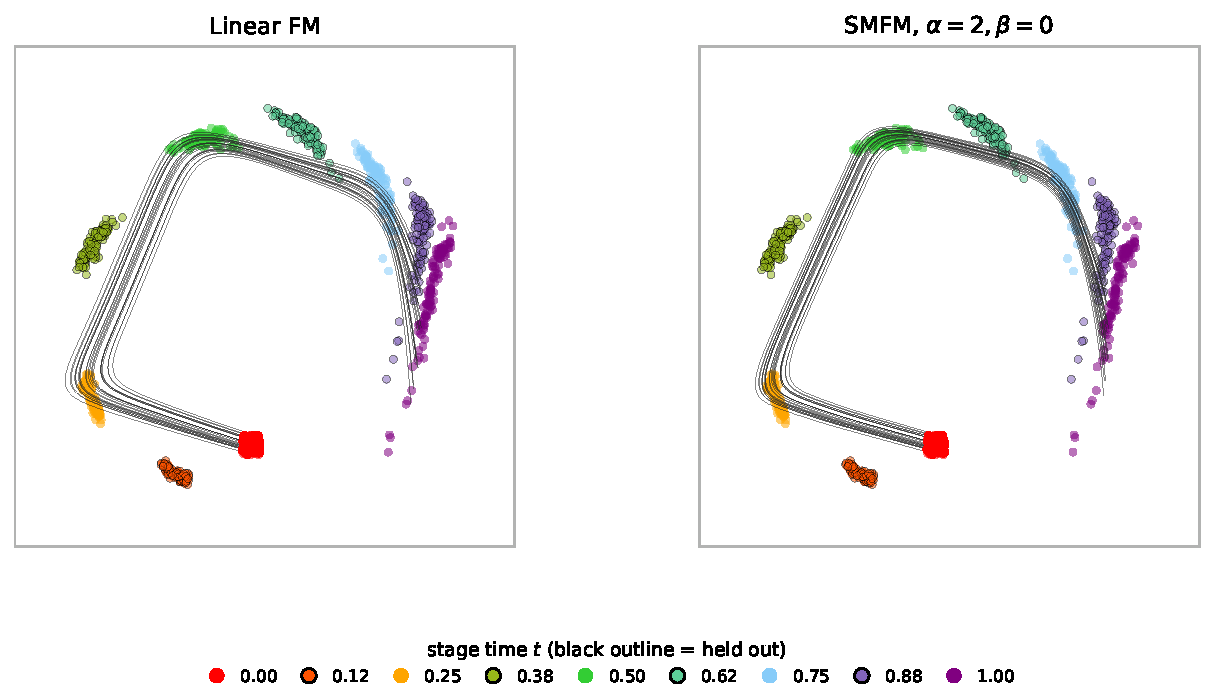
\includegraphics[width=0.7\linewidth]{figures/gom_trajectories.pdf}
\caption{GoM trajectories: Visualization of predicted trajectories on Gulf of Mexico simulated dataset. Left panel shows Linear FM with Euclidean optimal transport cost, right panel shows best \ourmodel sweeping $\alpha$ with $\beta=0$ fixed. Held-out marginals are shown with black outlines on the point. First marginal is red, last marginal is purple. The trajectories shown in both panels are predicted, all the points shown are the ground truth marginals.}
\label{fig:gom_trajectories}
\end{figure*}
\begin{table*}[t]
\centering
\caption{Per-stage chained $W_2$ on the Gulf of Mexico (GoM) 9-stage protocol with held-out marginals $\{1,3,5,7\}$. \ourmodel uses $\alpha=0.5$, $\beta=0$ with the Euclidean-cost kNN graph. Linear FM is the multi-marginal Euclidean baseline. Cells are mean$\,\pm\,$std over 5 splits $\times$ 5 init seeds.}
\label{tab:gom_otpfm9_w2}
\renewcommand{\arraystretch}{1.15}
\setlength{\tabcolsep}{6pt}
\begin{tabular}{lcccccc}
\toprule
Stage & $t$ & role & MM+Linear $W_2$ & \ourmodel $W_2$ & $\Delta\%$ \\
\midrule
$s_{1}$ & $0.12$ & held & $0.433\pm0.006$ & $0.429\pm0.004$ & $-0.9\%$  \\
$s_{2}$ & $0.25$ & train & $0.144\pm0.021$ & \textbf{$0.121\pm0.023$} & $-16.3\%$ \\
$s_{3}$ & $0.38$ & held & $0.825\pm0.019$ & \textbf{$0.477\pm0.033$} & $-42.1\%$  \\
$s_{4}$ & $0.50$ & train & $0.918\pm0.034$ & \textbf{$0.317\pm0.041$} & $-65.5\%$  \\
$s_{5}$ & $0.62$ & held & $0.989\pm0.031$ & \textbf{$0.401\pm0.053$} & $-59.4\%$  \\
$s_{6}$ & $0.75$ & train & $1.065\pm0.043$ & \textbf{$0.454\pm0.065$} & $-57.4\%$  \\
$s_{7}$ & $0.88$ & held & $1.176\pm0.067$ & \textbf{$0.556\pm0.068$} & $-52.7\%$  \\
$s_{8}$ & $1.00$ & train & $1.264\pm0.089$ & \textbf{$0.666\pm0.088$} & $-47.3\%$  \\
\midrule
\multicolumn{3}{l}{\emph{avg.\ over held-out marginals (1,3,5,7)}} & $0.856\pm0.026$ & \textbf{$0.466\pm0.036$} & $-45.5\%$  \\
\multicolumn{3}{l}{\emph{avg.\ over train marginals (0,2,4,6,8)}} & $0.848\pm0.035$ & \textbf{$0.390\pm0.043$} & $-54.1\%$  \\
\bottomrule
\end{tabular}
\end{table*}


\section{Discussion}
\begin{table*}[t]
\centering
\caption{Connectivity of datasets tested compared to improvement over baseline by using Spectral OT couplings with \ourmodel}
\label{tab:connectivity_outcome}
\renewcommand{\arraystretch}{1.18}
\setlength{\tabcolsep}{5pt}
\begin{tabular}{llrrrll}
\toprule
Dataset & Protocol & $D$ & $N_{\text{train}}$ & \#cc @ $k{=}15$ & Best $(\alpha,\beta)$ & $\Delta\%$ vs MM+Linear \\
\midrule
\multicolumn{7}{l}{\emph{Connected union graph $\Rightarrow$ spectral OT helps:}} \\
Pancreas      & 80/10/10                   & $2{,}000$ & $2{,}960$  & $1$ & $(\alpha{=}2.0,\,\beta{=}0)$    & $-24.4\%$         \\
Bone marrow   & 80/10/10                   & $2{,}000$ & $3{,}775$  & $1$ & $(\alpha{=}1.0,\,\beta{=}0)$    & $-44.3\%^{\star}$ \\
Paul15        & 80/10/10                   & $2{,}000$ & $1{,}262$  & $1$ & $(\alpha{=}0.0,\,\beta{=}0)$    & $-5.6\%^{\star}$  \\
Embryoid      & 80/10/10                   & $2{,}000$ & $24{,}827$ & $1$ & $(\alpha{=}1.0,\,\beta{=}0)$    & $-10.3\%^{\star}$ \\
\midrule
\multicolumn{7}{l}{\emph{Same encoding, broken temporal sampling $\Rightarrow$ spectral hurts; blend cannot rescue:}} \\
Embryoid      & hold-out $\{1,3\}$      & $2{,}000$ & $\sim\!1{,}500$ & $1$ & $(\alpha{=}0,\,\beta{=}0.25)$  & $-0.9\%^{\star}$  \\
\midrule
\multicolumn{7}{l}{\emph{Disconnected union graph $\Rightarrow$ performance depends on protocol:}} \\
GoM vortex    & 80/10/10                   & $2$       & $\sim\!500$    & $6$ & $(\alpha{=}0.5,\,\beta{=}0.0)$ & $-35.3\%^{\star}$ \\
GoM           & hold-out $\{1,3,5,7\}$  & $2$       & $\sim\!500$    & $6$ & $(\alpha{=}0.5,\,\beta{=}0.0)$ & $-45.5\%^{\star}$ \\
\midrule
\multicolumn{7}{l}{\emph{Severely disconnected (untested in the main grid):}} \\
Beijing PM2.5 & ---                        & $1$       & $9{,}409$      & $161$ & --- & ---                                \\
\bottomrule
\end{tabular}
\end{table*}


We find that spectral-cost OT helps most when the kNN graph over adjacent marginals is connective or otherwise informative about the geometric structure of the dataset (see Table \ref{tab:connectivity_outcome}. \ourmodel changes only the OT coupling cost and not the interpolation path or velocity field relative to the Linear FM baseline and shows improvements, dependent on the encoding of the data, on multiple datasets. This suggests that better pairings alone can improve multi-marginal Flow Matching. \cite{tongImprovingGeneralizingFlowbased2024} showed that switching from random pairings for FM training can increase stability and decrease inference time, we adapt this idea, by introducing the spectral-cost OT pairings based on the kNN graph Laplacian on the union of adjacent marginals. We find that the best $\alpha$ value (weighting which eigenvectors are used to compute spectral distance) differs by dataset, so the spectral scale $\alpha$ is a real hyperparameter to tune.

\section{Conclusion}
\label{ch:conclusion}
We introduced \ourmodel, a simple extension of multi-marginal Flow Matching that replaced the squared Euclidean ground cost used on OT couplings with graph-Laplacian spectral costs when pairing samples from adjacent marginals. This method keeps the simulation-free training objective and linear conditional paths of standard Flow Matching, while injecting information about the geometry of the data through the OT coupling step. Across the main connected-graph settings, the spectral OT couplings improve performance over the Linear FM baseline, suggesting that better OT pairings alone can improve multi-marginal FM.

The spectral-cost OT coupling approach we use in \ourmodel is orthogonal to many other approaches used in the past couple of years for multi-marginal Flow Matching models, such as the smooth spline-based interpolations used in MMFM \cite{rohbeckMODELINGCOMPLEXSYSTEM2025} or consistency models like MeanFlows \cite{gengMeanFlowsOnestep2025}. We propose using spectral-cost OT couplings as an addition to these models, when feasible, and investigating if it improves performance.

\paragraph{Future Work} We briefly tried but did not fully implement and investigate computing the graph spectral OT cost using a kNN graph over the entire dataset, instead of a kNN graph over adjacent marginals. We also propose but do not implement Riemannian Flow Matching using Optimal Transport couplings with squared geodesic distance ground cost.

\FloatBarrier
\clearpage
\raggedbottom
\onecolumn
\bibliographystyle{icml2026}
\bibliography{references}

\clearpage
\onecolumn
\appendix
\section{Additional Tables}
\label{app:additional_tables}
\FloatBarrier
\begin{table}[H]
\centering
\caption{Embryoid body 80/10/10, log1p HVG ambient + Euclidean kNN graph, subsampled to 2000 cells per stage. Chained MMD$^2$, mean$\pm$std over 5 splits $\times$ 5 init seeds.}
\label{tab:eb_8010_log1p_eucknn_2k}
\renewcommand{\arraystretch}{1.15}
\setlength{\tabcolsep}{4pt}
\begin{tabular}{lcccccc}
\toprule
& \multicolumn{4}{c}{MMD$^2$ at evaluation time / stage} & & \\
\cmidrule(lr){2-5}
Method & $t{=}0.25$ & $t{=}0.50$ & $t{=}0.75$ & $t{=}1.00$ & mean & $\Delta$ \\
\midrule
Linear FM
  & \underline{0.013}$\,\pm\,0.002$
  & \underline{0.023}$\,\pm\,0.003$
  & 0.025$\,\pm\,0.003$
  & 0.029$\,\pm\,0.003$
  & 0.023$\,\pm\,0.003$
  & --- \\
Random OT
  & 0.017$\,\pm\,0.001$
  & 0.025$\,\pm\,0.003$
  & 0.028$\,\pm\,0.003$
  & 0.028$\,\pm\,0.004$
  & 0.025$\,\pm\,0.002$
  & $+8.8\%$ \\
\ourmodel $\alpha=0$
  & 0.014$\,\pm\,0.002$
  & 0.024$\,\pm\,0.004$
  & 0.024$\,\pm\,0.003$
  & \textbf{0.026}$\,\pm\,0.001$
  & \underline{0.022}$\,\pm\,0.002$
  & $-3.6\%$ \\
\ourmodel $\alpha=0.5$
  & 0.013$\,\pm\,0.002$
  & 0.027$\,\pm\,0.002$
  & 0.024$\,\pm\,0.002$
  & \underline{0.027}$\,\pm\,0.002$
  & 0.023$\,\pm\,0.001$
  & $+1.0\%$ \\
\ourmodel $\alpha=1$
  & \textbf{0.013}$\,\pm\,0.001$
  & \textbf{0.020}$\,\pm\,0.003$
  & \textbf{0.021}$\,\pm\,0.003$
  & 0.027$\,\pm\,0.002$
  & \textbf{0.020}$\,\pm\,0.002$
  & $-10.3\%$ \\
\ourmodel $\alpha=1.5$
  & 0.013$\,\pm\,0.002$
  & 0.023$\,\pm\,0.005$
  & \underline{0.023}$\,\pm\,0.004$
  & 0.028$\,\pm\,0.004$
  & 0.022$\,\pm\,0.003$
  & $-3.2\%$ \\
\ourmodel $\alpha=2$
  & 0.014$\,\pm\,0.002$
  & 0.024$\,\pm\,0.004$
  & 0.025$\,\pm\,0.004$
  & 0.030$\,\pm\,0.003$
  & 0.023$\,\pm\,0.003$
  & $+2.1\%$ \\
\bottomrule
\end{tabular}
\end{table}

\begin{table}[H]
\centering
\caption{Paul15 erythroid trajectory (additional dataset), log1p HVG ambient + Euclidean kNN graph. Chained $\mathrm{MMD^2}$, mean $\pm$ std over 5 splits $\times$ 5 init seeds.}
\label{tab:paul15_log1p_eucknn}
\renewcommand{\arraystretch}{1.15}
\setlength{\tabcolsep}{4pt}
\begin{tabular}{lcccccc}
\toprule
& \multicolumn{4}{c}{MMD$^2$ at evaluation time / stage} & & \\
\cmidrule(lr){2-5}
Method & $t{=}0.25$ & $t{=}0.50$ & $t{=}0.75$ & $t{=}1.00$ & mean & $\Delta$ \\
\midrule
Linear FM
  & 0.108$\,\pm\,0.014$
  & 0.126$\,\pm\,0.021$
  & \underline{0.113}$\,\pm\,0.015$
  & \textbf{0.077}$\,\pm\,0.015$
  & \underline{0.106}$\,\pm\,0.015$
  & --- \\
Random OT
  & 0.106$\,\pm\,0.011$
  & \underline{0.118}$\,\pm\,0.016$
  & 0.122$\,\pm\,0.021$
  & 0.104$\,\pm\,0.026$
  & 0.112$\,\pm\,0.016$
  & $+6.0\%$ \\
\ourmodel $\alpha=0$
  & \textbf{0.101}$\,\pm\,0.010$
  & \textbf{0.115}$\,\pm\,0.012$
  & \textbf{0.106}$\,\pm\,0.008$
  & \underline{0.079}$\,\pm\,0.007$
  & \textbf{0.100}$\,\pm\,0.007$
  & $-5.6\%$ \\
\ourmodel $\alpha=0.5$
  & 0.108$\,\pm\,0.011$
  & 0.125$\,\pm\,0.010$
  & 0.126$\,\pm\,0.014$
  & 0.104$\,\pm\,0.019$
  & 0.116$\,\pm\,0.011$
  & $+8.9\%$ \\
\ourmodel $\alpha=1$
  & 0.108$\,\pm\,0.014$
  & 0.128$\,\pm\,0.014$
  & 0.136$\,\pm\,0.024$
  & 0.118$\,\pm\,0.025$
  & 0.123$\,\pm\,0.017$
  & $+15.8\%$ \\
\ourmodel $\alpha=1.5$
  & 0.105$\,\pm\,0.010$
  & 0.121$\,\pm\,0.011$
  & 0.119$\,\pm\,0.011$
  & 0.097$\,\pm\,0.017$
  & 0.110$\,\pm\,0.010$
  & $+4.1\%$ \\
\ourmodel $\alpha=2$
  & \underline{0.103}$\,\pm\,0.010$
  & 0.119$\,\pm\,0.011$
  & 0.115$\,\pm\,0.010$
  & 0.092$\,\pm\,0.014$
  & 0.107$\,\pm\,0.007$
  & $+1.4\%$ \\
\bottomrule
\end{tabular}
\end{table}

\begin{table}[H]
\centering
\caption{Pancreatic endocrinogenesis, Hellinger sphere encoding (alternate preprocessing). Chained $\mathrm{MMD^2}$, mean $\pm$ std over 5 splits $\times$ 5 init seeds.}
\label{tab:pe_sphere}
\renewcommand{\arraystretch}{1.15}
\setlength{\tabcolsep}{4pt}
\begin{tabular}{lcccccc}
\toprule
& \multicolumn{4}{c}{MMD$^2$ at evaluation time / stage} & & \\
\cmidrule(lr){2-5}
Method & $t{=}0.25$ & $t{=}0.50$ & $t{=}0.75$ & $t{=}1.00$ & mean & $\Delta$ \\
\midrule
Linear FM
  & \textbf{0.185}$\,\pm\,0.036$
  & 0.094$\,\pm\,0.018$
  & 0.159$\,\pm\,0.015$
  & 0.194$\,\pm\,0.014$
  & \textbf{0.158}$\,\pm\,0.015$
  & --- \\
Random OT
  & 0.232$\,\pm\,0.036$
  & 0.087$\,\pm\,0.006$
  & 0.164$\,\pm\,0.027$
  & \textbf{0.180}$\,\pm\,0.004$
  & 0.166$\,\pm\,0.011$
  & $+4.9\%$ \\
\ourmodel $\alpha=0$
  & 0.280$\,\pm\,0.036$
  & 0.103$\,\pm\,0.012$
  & 0.166$\,\pm\,0.017$
  & 0.227$\,\pm\,0.016$
  & 0.194$\,\pm\,0.009$
  & $+22.8\%$ \\
\ourmodel $\alpha=0.5$
  & \underline{0.210}$\,\pm\,0.042$
  & 0.101$\,\pm\,0.012$
  & 0.138$\,\pm\,0.011$
  & 0.240$\,\pm\,0.009$
  & 0.172$\,\pm\,0.014$
  & $+9.1\%$ \\
\ourmodel $\alpha=1$
  & 0.248$\,\pm\,0.045$
  & 0.078$\,\pm\,0.011$
  & \underline{0.138}$\,\pm\,0.026$
  & \underline{0.183}$\,\pm\,0.012$
  & 0.162$\,\pm\,0.018$
  & $+2.4\%$ \\
\ourmodel $\alpha=1.5$
  & 0.231$\,\pm\,0.039$
  & \textbf{0.071}$\,\pm\,0.016$
  & \textbf{0.122}$\,\pm\,0.016$
  & 0.213$\,\pm\,0.019$
  & \underline{0.159}$\,\pm\,0.019$
  & $+0.8\%$ \\
\ourmodel $\alpha=2$
  & 0.219$\,\pm\,0.040$
  & \underline{0.076}$\,\pm\,0.018$
  & 0.149$\,\pm\,0.014$
  & 0.248$\,\pm\,0.023$
  & 0.173$\,\pm\,0.019$
  & $+9.7\%$ \\
\bottomrule
\end{tabular}
\end{table}

\begin{table}[H]
\centering
\caption{Bone marrow, log1p HVG ambient + Euclidean kNN graph (alternate preprocessing). Chained $\mathrm{MMD^2}$, mean $\pm$ over 5 splits $\times$ 5 init seeds.}
\label{tab:bm_log1p_eucknn}
\renewcommand{\arraystretch}{1.15}
\setlength{\tabcolsep}{4pt}
\begin{tabular}{lcccccc}
\toprule
& \multicolumn{4}{c}{MMD$^2$ at evaluation time / stage} & & \\
\cmidrule(lr){2-5}
Method & $t{=}0.25$ & $t{=}0.50$ & $t{=}0.75$ & $t{=}1.00$ & mean & $\Delta$ \\
\midrule
Linear FM
  & 0.008$\,\pm\,0.001$
  & 0.027$\,\pm\,0.002$
  & \underline{0.051}$\,\pm\,0.003$
  & \textbf{0.083}$\,\pm\,0.006$
  & \textbf{0.042}$\,\pm\,0.002$
  & --- \\
Random OT
  & 0.009$\,\pm\,0.001$
  & 0.031$\,\pm\,0.002$
  & 0.053$\,\pm\,0.004$
  & 0.094$\,\pm\,0.007$
  & 0.047$\,\pm\,0.002$
  & $+10.9\%$ \\
\ourmodel $\alpha=0$
  & \textbf{0.007}$\,\pm\,0.001$
  & \textbf{0.025}$\,\pm\,0.002$
  & 0.053$\,\pm\,0.002$
  & \underline{0.086}$\,\pm\,0.005$
  & \underline{0.043}$\,\pm\,0.001$
  & $+1.2\%$ \\
\ourmodel $\alpha=0.5$
  & 0.007$\,\pm\,0.001$
  & \underline{0.026}$\,\pm\,0.002$
  & 0.057$\,\pm\,0.002$
  & 0.087$\,\pm\,0.005$
  & 0.044$\,\pm\,0.002$
  & $+5.1\%$ \\
\ourmodel $\alpha=1$
  & 0.009$\,\pm\,0.001$
  & 0.028$\,\pm\,0.002$
  & 0.054$\,\pm\,0.002$
  & 0.089$\,\pm\,0.004$
  & 0.045$\,\pm\,0.001$
  & $+6.2\%$ \\
\ourmodel $\alpha=1.5$
  & 0.008$\,\pm\,0.001$
  & 0.029$\,\pm\,0.002$
  & \textbf{0.051}$\,\pm\,0.002$
  & 0.088$\,\pm\,0.004$
  & 0.044$\,\pm\,0.001$
  & $+4.5\%$ \\
\ourmodel $\alpha=2$
  & \underline{0.007}$\,\pm\,0.001$
  & 0.027$\,\pm\,0.002$
  & 0.052$\,\pm\,0.002$
  & 0.091$\,\pm\,0.006$
  & 0.044$\,\pm\,0.001$
  & $+4.9\%$ \\
\bottomrule
\end{tabular}
\end{table}



\end{document}

% This document was modified from the file originally made available by
% Pat Langley and Andrea Danyluk for ICML-2K. This version was created
% by Iain Murray in 2018, and modified by Alexandre Bouchard in
% 2019 and 2021 and by Csaba Szepesvari, Gang Niu and Sivan Sabato in 2022.
% Modified again in 2023 and 2024 by Sivan Sabato and Jonathan Scarlett.
% Previous contributors include Dan Roy, Lise Getoor and Tobias
% Scheffer, which was slightly modified from the 2010 version by
% Thorsten Joachims & Johannes Fuernkranz, slightly modified from the
% 2009 version by Kiri Wagstaff and Sam Roweis's 2008 version, which is
% slightly modified from Prasad Tadepalli's 2007 version which is a
% lightly changed version of the previous year's version by Andrew
% Moore, which was in turn edited from those of Kristian Kersting and
% Codrina Lauth. Alex Smola contributed to the algorithmic style files.
